%----------------------------------------------------------------------------------------
%	PACKAGES AND THEMES
%----------------------------------------------------------------------------------------
\PassOptionsToPackage{table}{xcolor}
\documentclass[aspectratio=169,xcolor=dvipsnames,svgnames,x11names,fleqn]{beamer}
% \documentclass[aspectratio=169,xcolor=dvipsnames,fleqn]{beamer}

\usetheme{RedVelvet}

\usefonttheme[onlymath]{serif}
\newcommand{\showanswers}{yes}


\usepackage{xspace}
\usepackage{amsmath}
\usepackage{amssymb}
\usepackage{amsfonts}
\usepackage{color}
\usepackage{physics}
% \usepackage{mathbb}
\usepackage{rahul_math}
\usepackage{bigints}

\usepackage{graphicx} % Allows including images
\usepackage{booktabs} % Allows the use of \toprule, \midrule and \bottomrule in tables
\usepackage{tikz,pgfplots}

\usepackage{subfigure}
\usetikzlibrary{arrows}
\usepackage{minted}
\definecolor{LightGray}{gray}{0.9}
\definecolor{cream}{rgb}{0.92, 0.9, 0.55}
\definecolor{lightblue}{rgb}{0.68, 0.85, 0.9}


\usepackage{xcolor-material}
\usetikzlibrary{fit}
\usetikzlibrary{matrix}
\tikzset{%
apple/.pic={
    \fill [MaterialBrown] (-1/8,0)  arc (180:120:1 and 3/2) coordinate [pos=3/5] (@)-- ++(1/6,-1/7)  arc (120:180:5/4 and 3/2) -- cycle;
    \fill [MaterialLightGreen500] (0,-9/10)  .. controls ++(180:1/8) and ++(  0:1/4) .. (-1/3,  -1) .. controls ++(180:1/3) and ++(270:1/2) .. (  -1,   0) .. controls ++( 90:1/3) and ++(180:1/3) .. (-1/2, 3/4) .. controls ++(  0:1/8) and ++(135:1/8) .. (   0, 4/7)
    }
    }

\newcommand{\leftdoublequote}{\textcolor{blue}{\scalebox{3}{``}}}

\newcommand{\rightdoublequote}{\textcolor{blue}{\scalebox{3}{''}}}


\usepackage{textcomp}
\usepackage{fontawesome}
\usepackage{tikz,pgfplots}
\usetikzlibrary{shapes.callouts}
\usetikzlibrary{arrows}


\usepackage{overpic}

%----------------------------------------------------------------------------------------
%	TITLE PAGE
%----------------------------------------------------------------------------------------

\usepackage{tikz-qtree,tikz-qtree-compat}
\usetikzlibrary{tikzmark}
\usetikzlibrary{calc}


\title[CPE 486/586: Machine Learning]{CPE 486/586: Machine Learning for Engineers} % The short title appears at the bottom of every slide, the full title is only on the title page
\subtitle{08 Overfitting and Regularization}

\author[Rahul Bhadani] {{\Large \textbf{Rahul Bhadani}}}

\institute[UAH] % Your institution as it will appear on the bottom of every slide, maybe shorthand to save space
{
    Electrical \& Computer Engineering,  The University of Alabama in Huntsville
}
\date

% \titlegraphic{
%    \includegraphics[width=0.4\linewidth]{figures/UAH_primary.png}
% }

\begin{document}

%-------------------------------------------------
\begin{frame}
    \titlepage
\end{frame}

%-------------------------------------------------
\begin{frame}{Outline}
    \backgroundtableofcontents
\end{frame}



 
 %%%%%%%%%%%%%%%%%%%%%%%%%%%%%%%%%%%%%%%%%%%%%%%%%%%%%
\begin{sectionframe}{\faYelp}{Motivation}
\end{sectionframe}

\begin{frame}{Motivating Regularization}
    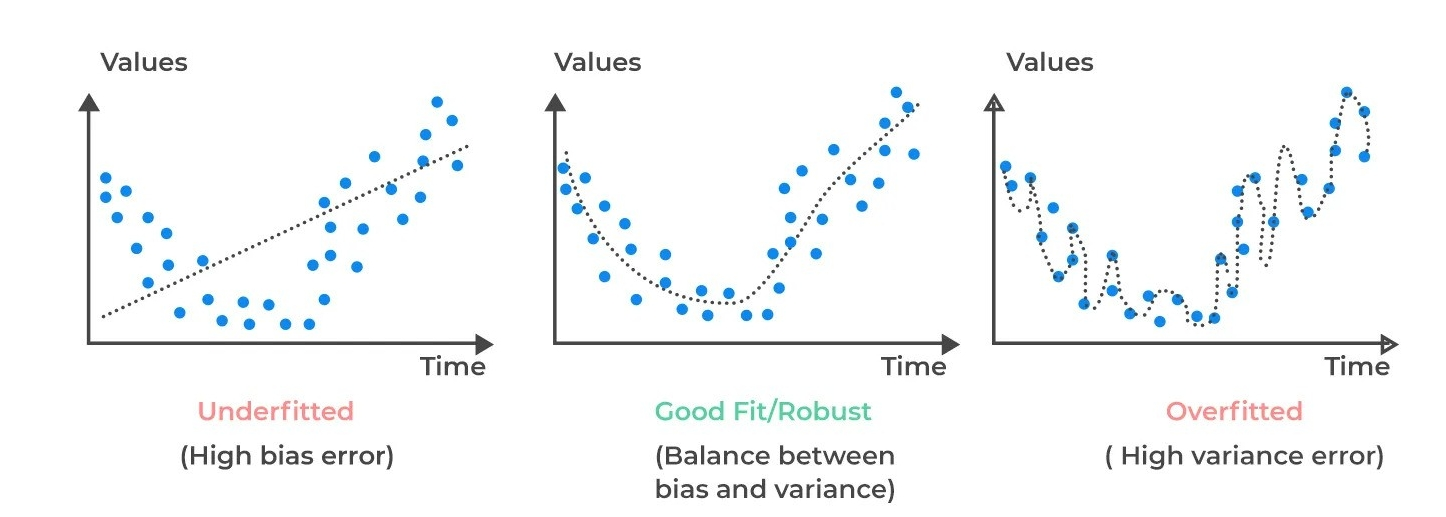
\includegraphics[width=0.99\textwidth]{figures/overfitting.jpg}
    
    \end{frame}

\begin{frame}{Underfitting}

        \begin{tblock}{}
        Underfitting occurs when a model is too simple to capture the underlying structure of the data. The model has high bias and low variance, leading to poor performance.
        \end{tblock}
\end{frame}
        

\begin{frame}{Overfitting}
    \begin{tblock}{}
    Overfitting occurs when a model is too complex and captures the noise along with the underlying structure of the data. The model has low bias and high variance, leading to good performance on training data but poor generalization to new data.
    \end{tblock}
    In overfitting the model describes random error or noise instead of the underlying relationship.
\end{frame}

\begin{frame}{Bias-Variance Trade-off}
    \begin{tblock}{}
    The bias-variance trade-off is the balance that must be found between the simplicity and complexity of a model. An optimal model complexity would result in low bias and low variance, minimizing total error.
    \end{tblock}
    


    \end{frame}

\begin{frame}{Bias}
    \begin{twilight}{}
        Bias is an error introduced in the model due to oversimplification of the algorithm used where data doesn't fit properly into the model. High-base is the case of underfitting.
    \end{twilight}
\end{frame}
    


\begin{frame}{Variance}
    \begin{ocean}{}
        Variance is the error introduced in the model due to a too-complex algorithm. It performs well on the training dataset but fails to generalize to unseen datasets (such as the test dataset).
    \end{ocean}
\end{frame}

\begin{frame}{}
    \begin{center}
            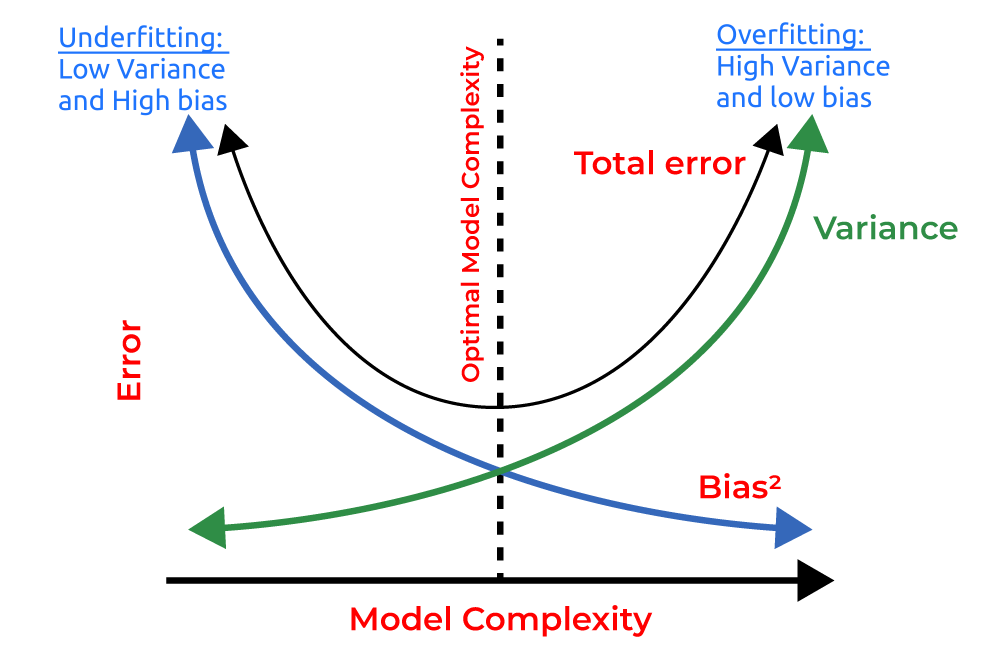
\includegraphics[width=0.79\textwidth]{figures/ML--Bias-Vs-Variance-.png}
    \end{center}
    
\end{frame}



%%%%%%%%%%%%%%%%%%%%%%%%%%%%%%%%%%%%%%%%%%%%%%%%%%%%%
\begin{sectionframe}{\faWrench}{Regularization}
\end{sectionframe}
    

\begin{frame}{What is Regularization}
    \begin{CloudNineBox}{}
        Regularization is a technique used in machine learning to prevent overfitting by adding a penalty term to the loss function. The penalty term discourages the learning algorithm from assigning too much importance to any individual feature, helping to keep the model simpler and more general.
    \end{CloudNineBox}
\end{frame}

\begin{frame}{Intuition Behind Regularization}
    \begin{origami}{}
        The intuition behind regularization is that simpler models are less likely to overfit. By adding a penalty term to the loss function, we encourage the learning algorithm to find simpler models that still fit the data well. This can lead to better generalization performance on unseen data.
    \end{origami}
\end{frame}
    
\begin{frame}[containsverbatim]{Linear Regression with $\ell_2$ Regularization}
    \Large
    \begin{tblock}{}
    \begin{multiequation}
        J(\wbf, w_0) &= {(\ybf - \xbf \wbf)^\T (\ybf - \xbf \wbf) } + \lambda \|\wbf\|_2^2 \\
        \frac{\partial J}{\partial\wbf} &=
        -\xbf^\T (\ybf - \xbf \wbf) + \lambda \Ibb \wbf= 0 \\
        (\xbf^\top \xbf + \lambda\Ibb)\wbf & = \xbf^\top \ybf\\
        &\longrightarrow \wbf = (\xbf^\T \xbf + \lambda\Ibb)^{-1} \xbf^\T \ybf
    \end{multiequation}
    \end{tblock}

\end{frame}

\begin{frame}{$\ell_2$ Penalty with Different $\lambda$}
    \begin{columns}
        \column{0.45\linewidth}
            \begin{center}
        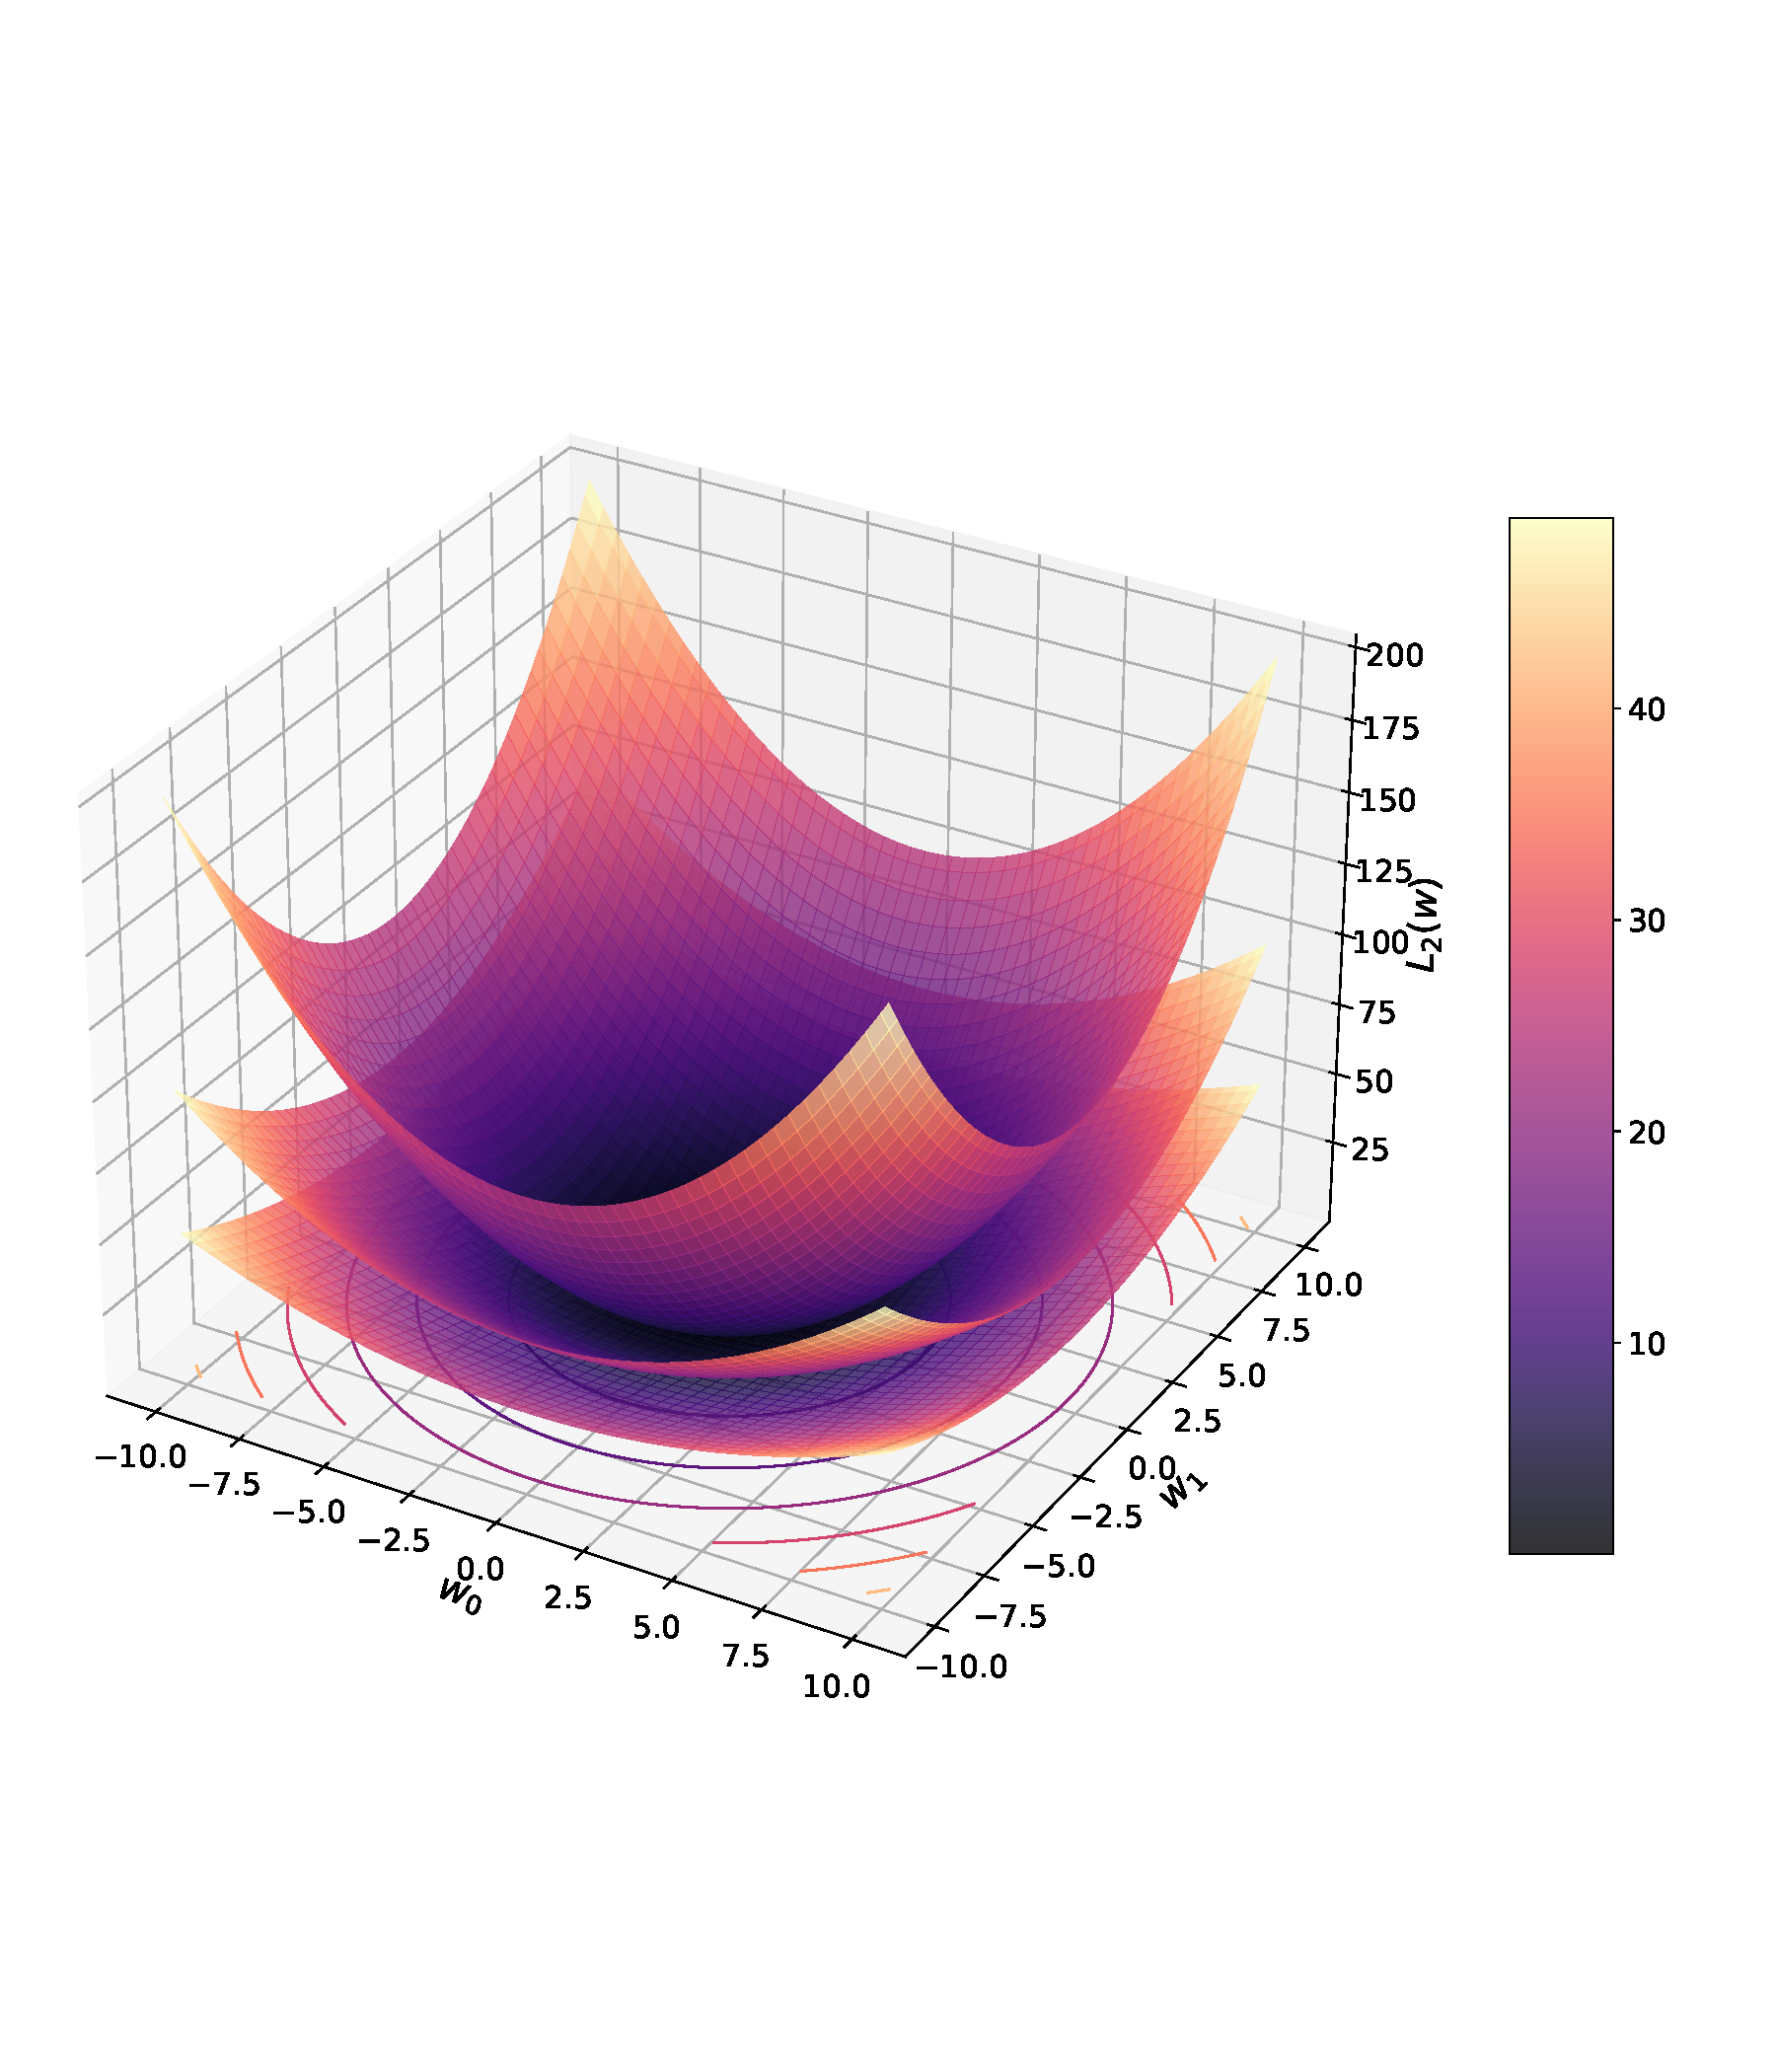
\includegraphics[width=1.0\textwidth]{figures/L2_Penalty.pdf}
    \end{center}
    \column{0.55\linewidth}
    \begin{itemize}
    \item The loss increases quadratically as the weights $w_0$ and $w_1$ move away from zero.  This encourages the optimization process to favor smaller weight values, effectively shrinking them toward zero.
        \item Smaller $\lambda$: The regularization term has little influence, and the optimization focuses more on minimizing the data fitting term. The $\ell_2$ surface becomes flatter, allowing larger weights.
        \item Larger $\lambda$: The regularization term dominates, forcing the weights closer to zero. The $\ell_2$ surface becomes steeper, strongly penalizing large weights.
    \end{itemize}
    \end{columns}
\end{frame}

\begin{frame}[containsverbatim]{$\ell_2$ Regularization in In Python}
    \begin{tblockFrost}{}
        \begin{minted}
            [
            framesep=1mm,
            baselinestretch=1.2,
            fontsize=\normalsize
            ]
            {python}
def linreg(X, y, reg:float=0.0): 
    return np.dot(np.dot(np.linalg.inv(np.dot(X.T, X) \ 
        + reg*np.eye(X.shape[1])), X.T), y)
        \end{minted}
    \end{tblockFrost}
\end{frame}

\begin{frame}{Regularized Linear Models: $g(\x) = \wbf^\T\x$}

    \begin{tblock}{Ridge Regression (Tikhonov regularization or $\ell_2$ regularization)}
        \Large
        \begin{multiequation}
            J_{RR} = \frac{1}{n} \sum_{i=1}^n (y_i - g(\x_i))^2
            + \lambda \sum_{j=1}^d w_j^2
        \end{multiequation}
    \end{tblock}
\end{frame}

% \begin{frame}[containsverbatim]{$\ell_2$ regularization in PyTorch}

%     \begin{tblockFrost}{}
%         \begin{minted}
%             [
%             framesep=1mm,
%             baselinestretch=1.2,
%             fontsize=\normalsize
%             ]
%             {python}
% def loss_fn(Y_hat, Y, lambda_reg, w0, w1):
%     mse = torch.mean((Y_hat - Y) ** 2)
%     l2_reg = lambda_reg * (torch.sum(w0 ** 2) + torch.sum(w1 ** 2))
%     return mse + l2_reg
%         \end{minted}
%     \end{tblockFrost}

% \end{frame}


\begin{frame}{Regularized Linear Models: $g(\x) = \wbf^\T\x$}
    %------------------------------------------------
    \begin{tblock}{LASSO or $\ell_1$ regularization}
    \Large
    \begin{multiequation}
        J_L = \frac{1}{n} \sum_{i=1}^n (y_i - g(\x_i))^2
        + \lambda \sum_{j=1}^d |w_j|
    \end{multiequation}
    \end{tblock}
    
    \end{frame}
    
    \begin{frame}{$\ell_1$ Penalty with Different $\lambda$}
        \begin{columns}
            \column{0.45\linewidth}
            \begin{center}
            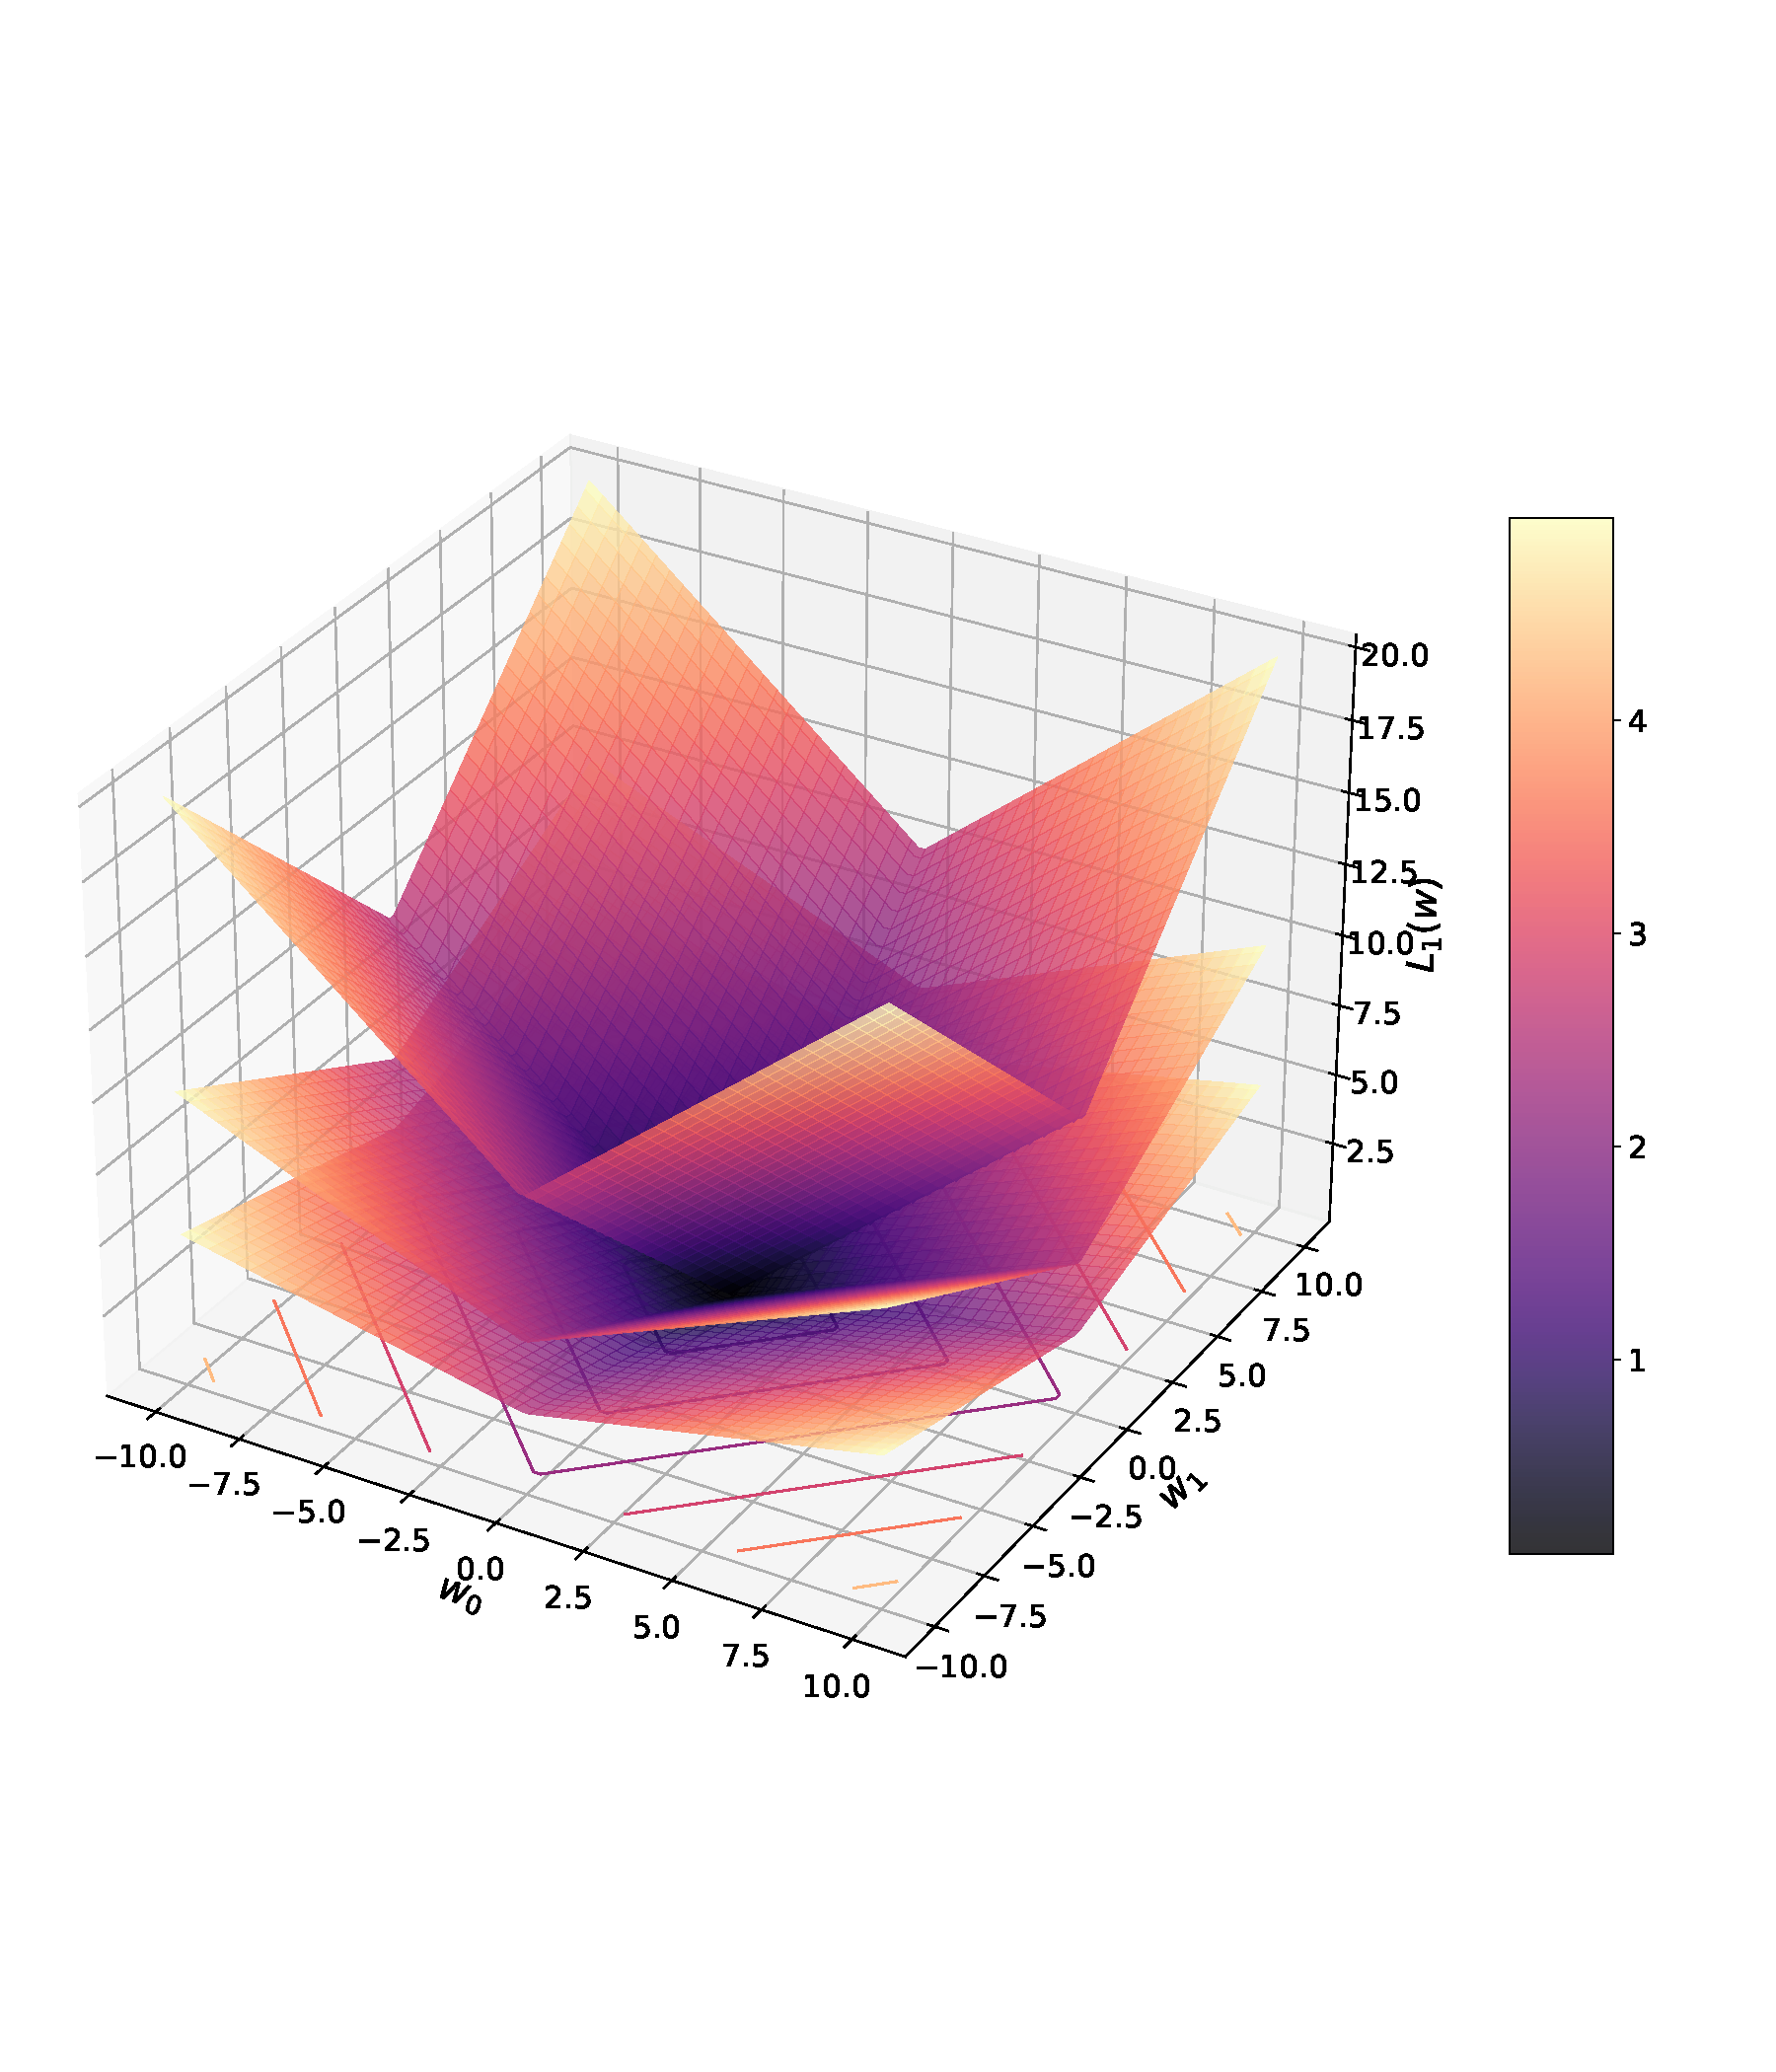
\includegraphics[width=1.0\textwidth]{figures/L1_Penalty.pdf}
        \end{center}
        \column{0.55\linewidth}
        \begin{itemize}
            \item The sharp edges and corners of the $\ell_1$ surface encourage weights to become exactly zero, promoting sparse solutions (a situation where most weights are zero).
            \item $\ell_1$ regularization is ideal for feature selection, as it eliminates irrelevant or less important features.
        \end{itemize}
        \end{columns}
    \end{frame}

    \begin{frame}{Regularized Linear Models: $g(\x) = \wbf^\T\x$}
        %------------------------------------------------
        \Large        
        \begin{tblock}{Elastic Nets}
        $\alpha \in [0,1]$
            \begin{multiequation}
                J_{EN} = \frac{1}{n} \sum_{i=1}^n (y_i - g(\x_i))^2
                + (1-\alpha)\lambda_2 \sum_{j=1}^d w_j^2
                + \alpha\lambda_1  \sum_{j=1}^d |w_j|
            \end{multiequation}
        \end{tblock}
    \end{frame}

\begin{frame}{Summary of Linear Regression}
    \begin{itemize}
        \item Linear, ridge, LASSO and elastic net regression are widely used in many fields for constructing a linear model. 
        \begin{itemize}
            \item LASSO and elastic nets can be used for feature selection too since many of the $w_j$'s will go to zero. 
            \item LASSO works best when $d\gg n$ and elastic nets should be used if $d >n$. 
        \end{itemize}
        \item Linear and ridge regression have closed for solutions; however, LASSO and elastic nets require that gradient-based methods be used to numerically find the solution. 
    \end{itemize}
\end{frame}
    
      %------------------------------------------------
    
    \begin{frame}[containsverbatim]{Python Notebook}
    \begin{center}
    \small
    { \color{Red}{\url{https://github.com/rahulbhadani/CPE486586_FA26/blob/master/Code/CPE486586_Ch08_Overfitting_And_Regularization.ipynb}}}
    \end{center}
    \end{frame}
    
    %------------------------------------------------
    
    \begin{frame}
        \Huge{\centerline{\color{MediumBlue}\textbf{The End}}}
    \end{frame}

\end{document}
